\documentclass[tikz,border=8pt]{standalone}
\usetikzlibrary{positioning,calc}
\begin{document}
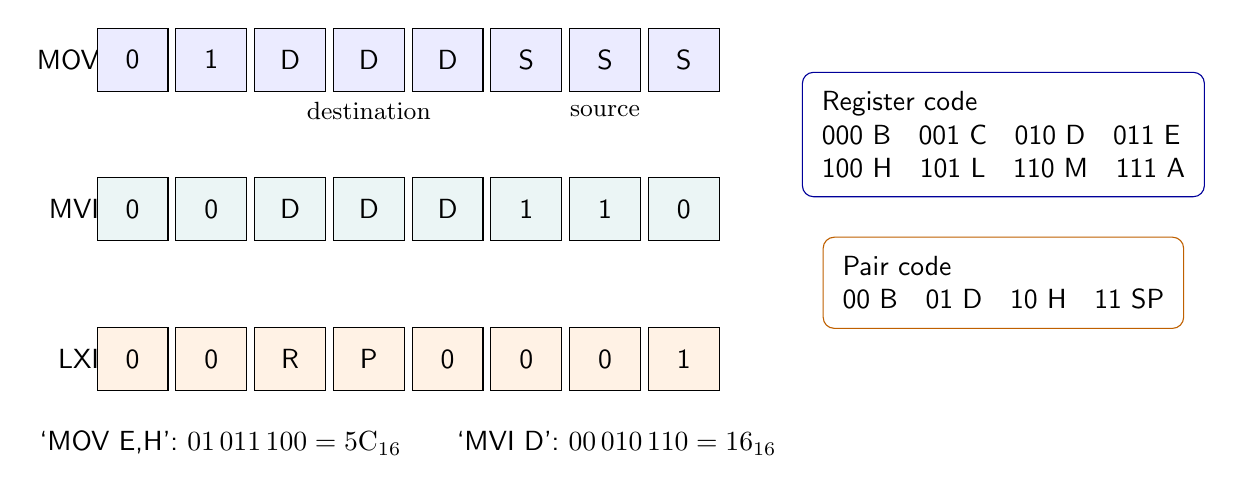
\begin{tikzpicture}[font=\sffamily,x=1cm,y=1cm,
bit/.style={draw,minimum width=9mm,minimum height=8mm,align=center},lab/.style={font=\small,align=center}]
\node[anchor=east] at (-.3,3.5){MOV};
\foreach \x/\v in {0/0,1/1,2/D,3/D,4/D,5/S,6/S,7/S}{\node[bit,fill=blue!8] at (\x,3.5){\v};}
\node[lab] at (3,2.85){destination};\node[lab] at (6,2.85){source};
\node[anchor=east] at (-.3,1.6){MVI};
\foreach \x/\v in {0/0,1/0,2/D,3/D,4/D,5/1,6/1,7/0}{\node[bit,fill=teal!8] at (\x,1.6){\v};}
\node[anchor=east] at (-.3,-.3){LXI};
\foreach \x/\v in {0/0,1/0,2/R,3/P,4/0,5/0,6/0,7/1}{\node[bit,fill=orange!10] at (\x,-.3){\v};}
\node[draw=blue!60!black,rounded corners,right=15mm of {$(7,1.6)!0.5!(7,3.5)$},align=left,inner sep=7pt] (r) {Register code\\000 B\quad001 C\quad010 D\quad011 E\\100 H\quad101 L\quad110 M\quad111 A};
\node[draw=orange!75!black,rounded corners,below=5mm of r,align=left,inner sep=7pt] {Pair code\\00 B\quad01 D\quad10 H\quad11 SP};
\node[below=8mm of {$(3.5,-.3)$},align=center] {`MOV E,H': $01\,011\,100=5\mathrm{C}_{16}$\qquad `MVI D': $00\,010\,110=16_{16}$};
\end{tikzpicture}
\end{document}
